\documentclass[11pt]{article}
\usepackage{amsmath, amssymb, mathtools}
\usepackage{listings}
\usepackage{xcolor}
\usepackage{mdframed}
\usepackage{graphicx}
\usepackage[utf8]{inputenc} % per interpretare i caratteri UTF-8
\usepackage[T1]{fontenc}    % per una corretta codifica dei font
\usepackage{float}


\lstset{
  language=Matlab,         % Linguaggio MATLAB
  basicstyle=\ttfamily\footnotesize, % Tipo di carattere (monospazio) e dimensione
  numbers=left,           % Numeri di riga a sinistra
  numberstyle=\tiny\color{gray}, % Stile numeri di riga
  stepnumber=1,           % Un numero per ogni riga
  numbersep=8pt,          % Distanza tra numeri di riga e codice
  backgroundcolor=\color{black!5}, % Sfondo leggermente grigio chiaro
  showstringspaces=false, % Non visualizzare spazi tra le stringhe
  keywordstyle=\bfseries\color{cyan!70!black}, % Parole chiave in blu-verde
  commentstyle=\itshape\color{green!50!black}, % Commenti in verde italico
  stringstyle=\color{red!80!black}, % Stringhe in rosso
  identifierstyle=\color{purple}, % Identificatori (variabili) in viola
  breaklines=true,        % Linee lunghe si spezzano
  frame=single,           % Cornice attorno al codice
  framexleftmargin=5pt,   % Distanza tra il codice e la cornice a sinistra
  framexrightmargin=5pt,  % Distanza tra il codice e la cornice a destra
  framextopmargin=5pt,    % Distanza tra il codice e la cornice in alto
  %framebottommargin=5pt,  % Distanza tra il codice e la cornice in basso
  rulecolor=\color{black}, % Colore della cornice
  captionpos=b,           % Posizione della didascalia (opzionale)
  aboveskip=10pt,         % Distanza sopra il blocco di codice
  belowskip=10pt,         % Distanza sotto il blocco di codice
  lineskip=2pt,           % Distanza tra le righe
}

% Impostazione per visualizzare i risultati della console
\lstdefinestyle{console}{
  basicstyle=\ttfamily\footnotesize\color{black},
  backgroundcolor=\color{black!10}, % Leggero grigio per il fondo
  frame=single,          % Cornice attorno ai risultati
  rulecolor=\color{black}, % Colore della cornice
  captionpos=b,           % Posizione della didascalia
  aboveskip=10pt,         % Distanza sopra il blocco di codice
  belowskip=10pt,         % Distanza sotto il blocco di codice
  numbers=none,           % No numerazione delle righe
  showstringspaces=false, % Non mostra gli spazi nelle stringhe
  breaklines=true,        % Le linee troppo lunghe si spezzano
}






\begin{document}

\title{Metodi di Risoluzione per ODE}

\author{Tobia Sacchetto}
\date{\today}
\maketitle

%%%%%%%%%%%%%%%%%%%%%%%%%%%%%%%%%%%%%%%%%%
\section{Esercizio 1}
%%%%%%%%%%%%%%%%%%%%%%%%%%%%%%%%%%%%%%%%%%
\subsection{Consegna}
Preso dall'esercizio 1: Considerare il metodo di Eulero esplicito e quello di Eulero implicito come la coppia di formule che forma un metodo predictor-corrector. Risolvere il seguente problema di Cauchy
\[
y'=-5y(x)+x \qquad y(0)=1
\]
sull’intervallo [0, 4] con passo $h = 0.1$. Indicare qual `e la costante di errore
(funzione di influenza) e fornirne una stima.

\subsection{Svolgimento}
\subsubsection{Svolgimento Teorico}
Si svolge il seguente integrale con il metodo di Eulero esplicito:\\
Si ricorda che $h=0.1=\frac{1}{10}$, di conseguenza $x_i=x_0+hi=0.1*i$, $\mu= \lfloor (x_1-x_0)/h+0.5) \rfloor = \lfloor(4-0)/0.1+0.5\rfloor=\lfloor40.5\rfloor=40$ e $i=0,...,40-1$, inoltre $y(0) \to x_0=0$, $f(x,y)=-5y+x$ e $y(0)=y_0=1$ . Per $y_i^{(1)}$ si intende l'iterato numero 1, il numero degli iterati nel codice è $p$ e per $i$ si intende il passo a cui ci si sta riferendo.
\begin{align*}
y_{(i+1)}^{(0)}&=y_i+h*f(x_i,y_i)\\
&=y_i+\frac{1}{10}(-5y_i+x_i)\\
&=y_i-\frac{1}{2}y_i+\frac{1}{10}x_i\\
&=\frac{1}{2}y_i+\frac{1}{100}i
\end{align*}
Questo lo si sostituisce con $y_{i+1}^{(0)}$ nel metodo Eulero implicito (per $p=1$).
\begin{align*}
	y_{(i+1)}^{(1)}&=y_i+h\cdot f(x_{i+1},y_{i+1}^{(0)})\\
	&=y_i+\frac{1}{10}\cdot (-5\cdot (\underbrace{\frac{1}{2}y_i+\frac{1}{100}i}_{y^{(0)}_{i+1}})+\underbrace{(i+1) \cdot\frac{1}{10}}_{x_{i+1}})\\
	&=y_i+ \frac{1}{10}\cdot(-\frac{5}{2}y_i-\frac{1}{20}i+\frac{1}{10}i+\frac{1}{10})\\
	&=y_i-\frac{1}{4}y_i+\frac{1}{200}i+\frac{1}{100}\\
	&=\frac{3}{4}y_i+\frac{1}{200}i+\frac{1}{100}
\end{align*}
Ora lo si svolge per $p=2$ (Sempre con Eulero implicito)
\begin{align*}
	y_{i+1}^{(2)}&=y_i+h\cdot f(x_{i+1},y_{i+1}^{(1)})\\
	&=y_i+\frac{1}{10}\cdot (-5\cdot (\underbrace{\frac{3}{4}y_i+\frac{1}{200}i+\frac{1}{100}}_{y^{(1)}_{i+1}})+\underbrace{(i+1) \cdot\frac{1}{10}}_{x_{i+1}})\\
	&=y_i+\frac{1}{10}\cdot (-\frac{15}{4}y_i-\frac{1}{40}i-\frac{1}{20}+\frac{1}{10}i+\frac{1}{10})\\
	&=y_i -\frac{3}{8}y_i+\frac{3}{400}i+\frac{1}{200}\\
	&=\frac{5}{8}y_i+\frac{3}{400}i+\frac{1}{200}
\end{align*}
\subsubsection{Svolgimento Pratico}
Segue il codice MATLAB per constatare se si sono eseguiti i calcoli del punto precedente nel modo corretto. Si tiene a ricordare che corrector è Eulero implicito, mentre il predictor è Eulero esplicito. Viene fatto uso della funzione eulero\_implicito\_mod.\\
Funzione eulero\_implicito\_mod:\\
\begin{lstlisting}
function [y_esp,y_impl]=eulero_implicito_mod(f,y0,x0,x1,h,p) %p=numero di passi in cui voglio effettuare il corrector (quanto preciso deve essere)

x=x0:h:x1; %numero di nodi
y = zeros(length(x), length(y0));
y_esp = zeros(length(x), length(y0));
y_impl = zeros(length(x), length(y0));
y(1,:)=y0;

for i=1:length(x)-1
    %predictor
    pre=y(i,:)+h*feval(f,x(i),y(i,:)); %eulero esplicito in cui do in pasto come precedente il corrector
    y_esp(i,:)=pre;
    %corrector
    for k=1:p
        pre=y(i,:)+h*feval(f,x(i+1),pre); %eulero implicito
    end
    y(i+1,:)=pre;
end
%ultimo valore per il predictor che non ho
i=length(x);
y_esp(i,:)=y(i,:)+h*feval(f,x(i),y(i,:)); 
   
y_impl=y;
\end{lstlisting}
Main Es\_1:\\
\begin{lstlisting}
close all
clear all
clc 
addpath("/Users/tobiasacchetto/Documents/GitHub/Numerical_Analysis_II/matlab_class_exercises/Function");

h=0.1; %passo
x0=0; x1=4; %intervalli
x=x0:h:x1; %x esplicita
p = 2; %quanto voglio preciso il corrector
y0=1;
f=@(x,y)(-5*y+x);

%soluzione esatta
exact_sol=@(x)((5*x-1)/25+(24/25)*exp(-5*x));
exact_soll=arrayfun(exact_sol,x);
%chiamo eulero implicito / esplicito
[y_explicit,y_implicit]=eulero_implicito_mod(f,y0,x0,x1,h,p);
y_eulero=eulero(f,y0,x);




%% 3. CONFRONTO VISIVO DEI RISULTATI
figure;
plot(x, y_explicit, 'b-o', 'LineWidth', 1.5, 'DisplayName', 'Predictor(Eulero Esplicito)');
hold on;
plot(x, exact_soll, 'g-o', 'LineWidth', 1.5, 'DisplayName', 'Soluzione Esatta');
plot(x, y_implicit, 'r-s', 'LineWidth', 1.5, 'DisplayName', 'Corrector(Eulero Implicito) p=2');
plot(x, y_eulero, 'm-s', 'LineWidth', 1.5, 'DisplayName', 'Eulero Esplicito');
[y_explicit,y_implicit_p1]=eulero_implicito_mod(f,y0,x0,x1,h,1);
plot(x, y_implicit_p1, 'y-s', 'LineWidth', 1.5, 'DisplayName', 'Corrector(Eulero Implicito) p=1');
xlabel('x');
ylabel('y(x)');
title('Confronto tra metodi di Eulero');
legend('show');
grid on;


fprintf('\nPrimi 5 valori:\n');
fprintf('  i      x(i)     Esatta      Eulero Exp.   Predictor (p=2)   Corrector (p=2)   Corrector (p=1)\n');
fprintf('----------------------------------------------------------------------------------------------\n');
for i = 1:5
    fprintf('%3d   %7.2f   %9.5f   %10.5f     %10.5f       %10.5f       %10.5f\n', ...
        i-1, x(i), exact_soll(i), y_eulero(i), y_explicit(i), y_implicit(i), y_implicit_p1(i));
end
\end{lstlisting}
\subsection{Confronto Risultati}
I risultati che vengono dati da MATLAB sono uguali a quelli che sono stati calcolati. Il plot che lo script stampa è il seguente. Esso mette a confronto i vari metodi con la soluzione esatta.
\begin{figure}[H]
  \centering
  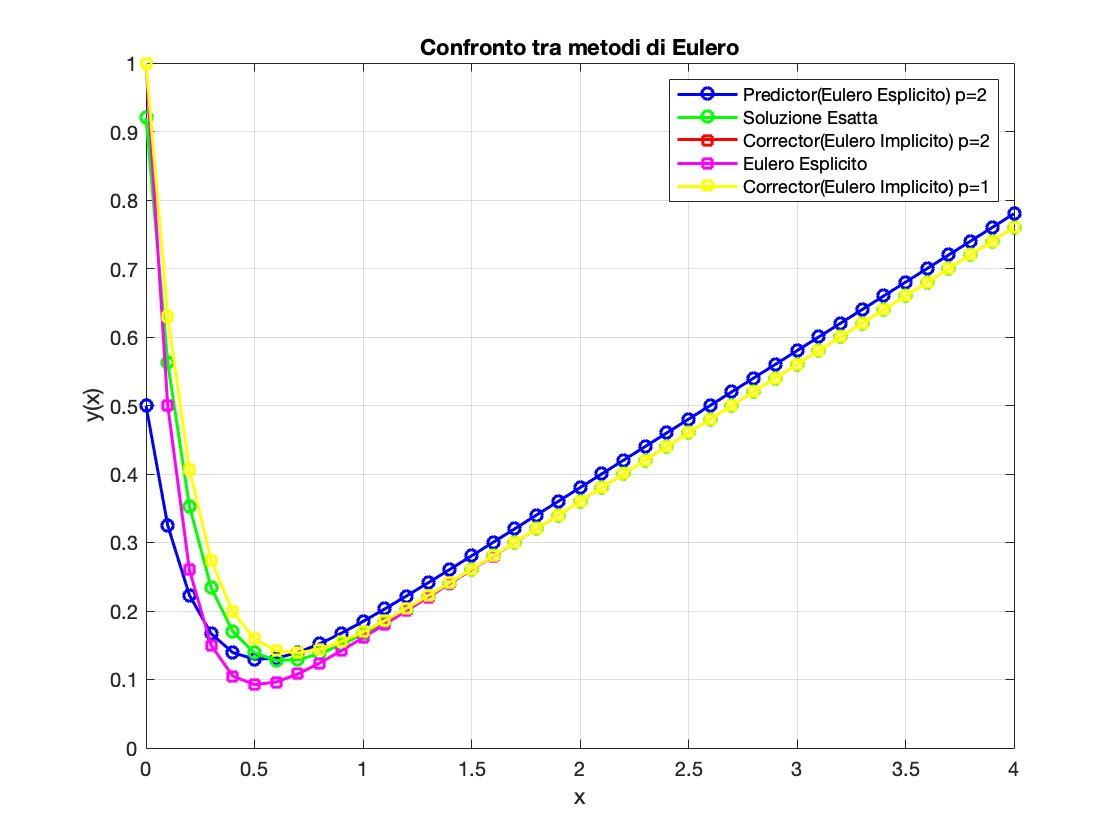
\includegraphics[width=0.7\textwidth]{images/fig1.jpg} 
  \caption{Confronto fra i vari metodi}
  \label{fig:funzione}
\end{figure}
\subsection{Errore}
Formula generale per l'errore globale:
\[
E_n=\sum^{n-1}_{k=0}I_{n,k}\tau_k
\]
dove $I_{n,k}$ è la funzione di influenza in cui l'errore locale passo $k$ influisce l'errore globale al passo $n$. La funzione nel caso di Eulero implicito è:
\[
I_{n,k}=\prod^{n-1}_{j=k+1}\frac{1}{1-h\cdot f_y(x_{j+1},y(x_{j+1}))}
\]
quindi $f_y(x_{j+1},y(x_{j+1}))$ è la derivata parziale di $f$ rispetto $y$ nel punto $(x_{j+1},y(x_{j+1}))$ e di conseguenza
\begin{align}
	I_{n,k}&=\prod^{n-1}_{j=k+1}\frac{1}{1-h(-5)}\\
	&=\prod^{n-1}_{j=k+1}\frac{1}{1+ \frac{1}{2}}\\
	&=\prod^{n-1}_{j=k+1}\frac{2}{3}\\
	&=\left( \frac{2}{3}\right)^{n-k-1}
\end{align}
L'errore locale $\tau_k$, per Eulero implicito è di ordine $h^2$ ed è tipicamente:
\[
\tau_{k+1} = \frac{h^2}{2} y''(\xi_k) \quad \text{per qualche } \xi_k \in (x_k, x_{k+1})
\]
SI svolge prima $y''(\xi_k)$. Nel problema si ha:
\[
y'=-5y+x \Rightarrow y''=-5y'+1=25y-5x+1
\]
Usando la soluzione esatta $y(x)=\frac{5x-1}{25}+\frac{24}{25}e^{-5x}$ si ottiene:
\[
y''(x)=24e^{-5x}
\]
Quindi
\begin{align}
	|\tau_{k+1}|&\leq \frac{h^2}{2} 24e^{-5x}\\
	&\leq h^212e^{-5x}\\
	&\leq \left(\frac{1}{10}\right)^212e^{-5x}\\
	&\leq \frac{3}{25}e^{-5x}
\end{align}
La funzione che si ricava è una funzione monotona decrescente.
\begin{figure}[H]
  \centering
  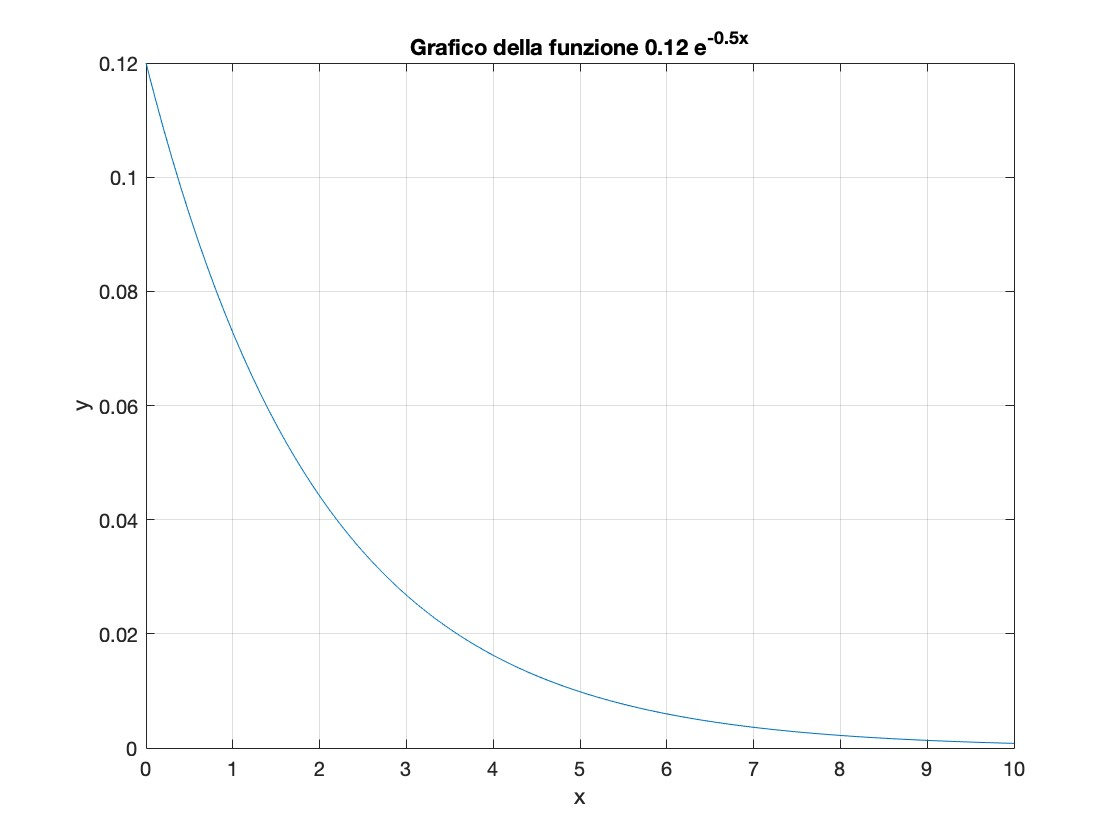
\includegraphics[width=0.7\textwidth]{images/fig2.jpg} 
  \caption{Errore di troncamento}
  \label{fig:funzione}
\end{figure}
\subsubsection{Errore globale: Ipotesi 1} 
Ora si riesce a calcolare una stima dell'errore globale. Si assume che l'errore di troncamento sia limitato uniformemente per $\tau_k\leq 0.12$ (si prende l'elemento maggiore possibile):
\[
E_n\leq\sum^{n-1}_{k=0}\left(\frac{2}{3} \right)^{n-k-1}0.12
\]
Posto $m=n-k-1$, quando $k=0,m=n-1$; quando $k=n-1, m=0$. Dunque la serie diventa una serie geometrica:
\[
\sum^{n-1}_{m=0}\left( \frac{2}{3} \right) ^{m}=\frac{1-\left( \frac{2}{3} \right) ^n}{1-\frac{2}{3}}=3 \left( 1- \left( \frac{2}{3} \right)^n \right)
\]
Quindi la stima diventa:
\[
E_n\leq0.12\cdot3 \left( 1- \left( \frac{2}{3} \right)^n \right)=0.36 \left( 1- \left( \frac{2}{3} \right)^n \right)\leq0.36
\]
Questo non dipende da $n$. Sarà sempre limitato $\leq0.36$. Si mostra la funzione:
\begin{figure}[H]
  \centering
  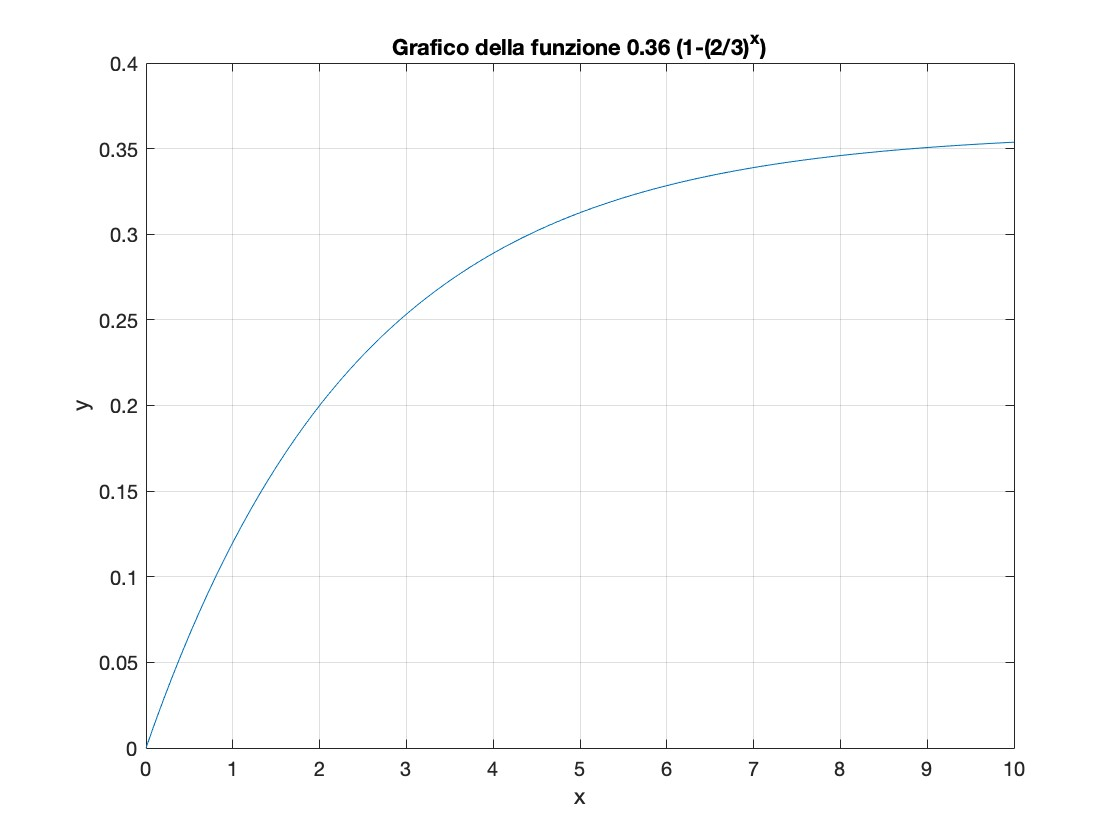
\includegraphics[width=0.7\textwidth]{images/fig3.jpg} 
  \caption{L'errore globale Ipotesi 1}
  \label{fig:funzione}
\end{figure}
\subsubsection{Errore Globale: Ipotesi 2}
Si assume, in questo caso, che l'errore di troncamento decada esponenzialmente $\tau_k\leq12h^2e^{-0.5k}$. Quindi si ha una funzione più precisa per l'errore di troncamento rispetto l'ipotesi 1. Quindi:
\begin{align}
	E_n&\leq12h^2\sum^{n-1}_{k=0}\left(\left(\frac{2}{3} \right)^{n-k-1}e^{-\frac{1}{2}k}\right)\\
	&\leq12h^2\left(\frac{2}{3} \right)^{n-1}\sum^{n-1}_{k=0}\left(\left(\frac{3}{2} \right)^{k}e^{-\frac{1}{2}k}\right)\\
	&\leq12h^2\left(\frac{2}{3} \right)^{n-1}\sum^{n-1}_{k=0}\left(\left(\frac{3}{2} \right)^{k}e^{-\frac{1}{2}k}\right)\\
	&\leq12h^2\left(\frac{2}{3} \right)^{n-1}\sum^{n-1}_{k=0}\left(\left( \frac{3}{2}e^{-\frac{1}{2}}\right)^k\right)
\end{align}
Si nota che $\frac{3}{2}e^{-\frac{1}{2}}\approx0.9098$ e si trova una serie geometrica $\sum^{n-1}_{k=0}0.9098^k\approx\frac{1}{1-0.9098}$. Dunque:
\begin{align}
	E_n&\leq12h^2\left(\frac{2}{3} \right)^{n-1}\frac{1}{1-0.9098}\\
	&\leq12\left(\frac{1}{10}\right)^2\left(\frac{2}{3} \right)^{n-1}\frac{1}{1-0.9098}\\
	&\leq\frac{3}{25}\left(\frac{2}{3} \right)^{n-1}\frac{1}{0.0902}
\end{align}
Quindi $E_n$ decade per $\left(\frac{2}{3}\right)^{n-1}$. Si mostra un grafico rappresentativo della funzione dell'errore globale più accurato dell'ipotesi 1.
\begin{figure}[H]
  \centering
  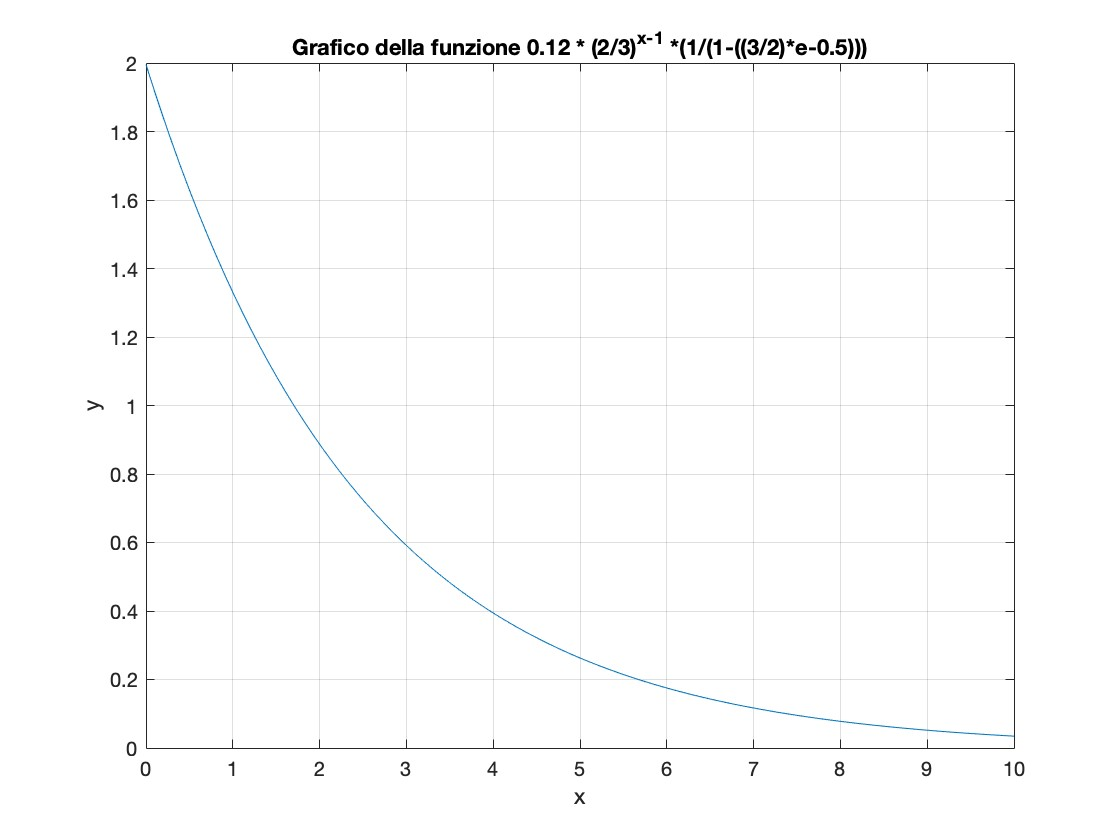
\includegraphics[width=0.7\textwidth]{images/fig4.jpg} 
  \caption{L'errore globale Ipotesi 2}
  \label{fig:funzione}
\end{figure}
Per $h=0.1$ e $n=40$, cioè $x=4$ risulta una stima numerica molto piccola dell'ordine di $10^{-7}$. Da notare che l'errore massimo che si può avere si verifica all'inizio ($n=0$) e tende a decrescere.
\section{Esercizio 2}
\subsection{Consegna}
Preso da esercizio 3. Dato il metodo di Runge Kutta a tre stadi:
\begin{align}
	y_{i+1}&=y_i+\frac{h}{9}(2K_1+3K_2+4K_3)\\
	K_1&=f(x_i,y_i)\\
	K_2&=f(x_i+\frac{h}{2} ,y_i+\frac{h}{2}K_1)\\
	K_3&=f(x_i+\frac{3h}{4} ,y_i+\frac{3h}{4}K_2)
\end{align}
risolvere con tale metodo il problema $y'=-34y$,   $y(0)=1$ sull’intervallo $[0, 1]$, scegliendo il passo in modo da avere assoluta stabilità.\\
Ripetere usando la regola trapezoidale abbinata ad un conveniente passo (discutere la selezione fatta del passo).
\subsection{Svolgimento}
\subsubsection{Risoluzione numerica tramite Runge-Kutta}
Con $f(x, y)=-34y$ [attenzione, non dipende dalla $x$, quindi l'intero termine $(x_i+h/2)$ non c'è. Se fosse stato $f(x, y)=x+y$ allora si avrebbe $K_2=(x_i+h/2)+(y_i(1-17h))$ ], si ottiene :
\begin{align}
K_1&=f(x_i, y_i)\\
	&=-34y_i\\
	K_2&=f(x_i+\frac{h}{2} ,y_i+\frac{h}{2}K_1)\\
	y^{(1)}&=y_i+\frac{h}{2}K_1\\
	&=y_i+\frac{h}{2}(-34y_i)\\
	&=y_i(1-17h)\\
	K_2&=f(x_i+\frac{h}{2} ,y^{(1)})\\
	&=-34(y_i(1-17h))\text{ Si ricorda che $f(x,y)=-34y$}\\
\end{align}
\begin{align}
	K_3&=f(x_i+\frac{3h}{4} ,y_i+\frac{3h}{4}K_2)\\
	&=-34(y_i+\frac{3h}{4}K_2)\\
	&=-34(y_i+\frac{3h}{4}(-34y_i(1-17h)))\\
	&=-34y_i(1+\frac{3h}{4}(-34)(1-17h))\\
	&=-34y_i(1+\frac{3h}{4}(-34+578h))\\
	&=-34y_i(1-\frac{51h}{2}+\frac{867h^2}{2})\\
	y_{i+1}&=y_i\frac{h}{9}(2K_1+3K_2+4K_3)\\
	&=y_i\frac{h}{9}(2(-34y_i)+3(-34(y_i(1-17h)))+4(-34y_i(1-\frac{51h}{2}+\frac{867h^2}{2})))\\
	&=y_i\frac{h}{9}\cdot(-34y_i)(9-153h+1734h^2)
\end{align}
Per Runge-Kutta a 3 stadi (esplicito) per trovare il passo $h$ si deve prima trovare la funzione di stabilità sul test lineare $y' = \lambda y$ che è data dal polinomio di grado 3 ottenuto troncando la serie di Taylor di $e^z$:
\[
R(z) = 1 + z + \frac{z^2}{2} + \frac{z^3}{6}, \quad \text{dove } z = h\lambda.
\]
Il dominio di stabilità assoluta sul semiasse reale negativo è un intervallo:
\[
z \in (\alpha, 0),
\]
Il metodo è assolutamente stabile per quei valori di $z$ per cui:
\[
|R(z)| \leq 1.
\]
Siccome $\lambda = -34 < 0$, ci si concentra solo sul semiasse reale negativo $z \in (-\infty, 0)$. Quindi si deve determinare fino a quale valore negativo di $z$ si ha:
\[
|R(z)| \leq 1.
\]
Cioè, si deve trovare l'estremo sinistro dell'intervallo di stabilità assoluta del metodo, ovvero il valore $\alpha < 0$ tale che:

\[
|R(z)| \leq 1 \quad \text{per ogni } z \in (\alpha, 0),
\]

dove $R(z)$ è la funzione di stabilità:

\[
R(z) = 1 + z + \frac{z^2}{2} + \frac{z^3}{6}.
\]
Ora si moltiplica tutto per 6. Si ricorda inoltre che il bordo sinistro del dominio di stabilità reale si ottiene risolvendo: $R(z)=-1$. Dunque:
\begin{align}
	-1 &= 1 + z + \frac{z^2}{2} + \frac{z^3}{6}\\
	-6 &= 6 + 6z + 3z^2 + z^3\\
	0&= 12+ 6z + 3z^2 + z^3
\end{align}
Si usa il metodo di Newton globale (sis\_newton\_glob) per risolvere l'equazione non lineare definita dalla funzione:
\[
p(z)=z^3 + 3z^2 + 6z +12
\]
con derivata:
\[
p'(z)=3z^2 + 6z + 6
\]
Es2:
\begin{lstlisting}
close all
clear all
clc

% Definizione funzione p(z)
pz = @(x)( x.^3 + 3*x.^2 + 6*x + 12);

% Derivata p'(z)
dpz= @(x)(3*x.^2 + 6*x + 6);


% Chiamata al metodo di Newton globale
x0 = -4;           % punto iniziale (es. vicino a una radice reale)
tolx = 1e-10;
tolf = 1e-10;
maxit = 100;

[x,it,iterati,merito] = sis_newton_glob(pz, dpz, x0, tolx, tolf, maxit);
fprintf('Radice trovata: %.12f in %d iterazioni\n', x, it);

\end{lstlisting}
\begin{lstlisting}
sis_newton_glob:
function [x,it,iterati,merito] = sis_newton_glob(fvett,jac,x0,tolx,tolf,maxit)
%Parametri per cui dipende il metodo
beta=1e-4; %va cosi' di default sempre di solito
rho=0.5;
delta=0.01;
%%%%%
x=x0(:);
n=length(x);
iterati{1}=x;
f=feval(fvett,x);
J=feval(jac,x);
merito=zeros(maxit,1);
merito(1)=0.5*norm(f)^2;
for it=1:maxit
    dx=J\(-f); %J dx=-f
    gradmerito=J'*f;
    tau=1;
    dirdis=gradmerito'*dx;
    costheta=abs(dirdis)/(norm(gradmerito)*norm(dx));
    while costheta <= delta
        [Q,R]=qr([J; sqrt(tau)*eye(n)]);
        R=R(1:n,:);
        dx=R\(R'\(-gradmerito));
        dirdis=gradmerito'*dx;
        tau=tau*10;
    end
    %Ok e' come se stessimo partendo come se alpha fosse uguale a 1
    f0=f;
    x0=x;
    alpha=1;
    normf0=norm(f0)^2;
    x=x0+alpha*dx;
    f=feval(fvett,x);
    while norm(f)^2>(1-2*beta*alpha)*normf0
        alpha=alpha*rho;
        x=x0+alpha*dx;
        f=feval(fvett,x);
    end
    iterati{it+1}=x;
    merito(it+1)=1/2*norm(f)^2;
    if (norm(dx,inf)<=eps+tolx*norm(x,inf)) && (norm(f,inf)<=tolf)
        break
    end 
    J=feval(jac,x);
end
if it>=maxit
    fprintf('raggiunto massimo numero di iterazioni\n');
end
\end{lstlisting}
\begin{lstlisting}[style=console]
	Radice trovata: -2.512745326618 in 6 iterazioni
\end{lstlisting}
Per trovare $\lambda$ si segue la formula:
\begin{align}
	y'&=\lambda y\\
	&=-34y\\
	\lambda&=-34
\end{align}

Quindi si è trovato $\alpha \approx -2.5127453$. Per garantire che tutti i punti 
\[
z = h\lambda \quad \text{(con } \lambda = -34 \text{)}
\]
appartengano all'intervallo di stabilità assoluta
\[
z \in (\alpha, 0), \quad \text{con } \alpha \approx -2.5127453,
\]
è necessario che:

\[
h|\lambda| \leq 2.5127453 \quad \Longrightarrow \quad h \leq \frac{2.5127453}{34} \approx 0.07390.
\]
Quindi, qualsiasi passo
\[
h \leq 0.07390
\]
assicura la stabilità assoluta del metodo per il problema.
Si pone come passo $h=\frac{1}{14}\approx0.0714286$ che è minore del limite di stabilità $0.07390$ e di conseguenza il metodo risulta stabile. Si pone $y_i=1$
\begin{align}
	K_1&=-34y_i=-34\\
	K_2&=-34(1-17\frac{1}{14})\\
	&=-34\left(\frac{3}{14} \right)=\frac{51}{7}\approx7.2857142857\\
	K_3&=-34\left(\frac{545}{392}\right)=-\frac{9265}{196}\approx-47.2704081633\\
	y_{i+1}&=\frac{h}{9}\cdot(-34)(9-153\frac{1}{14}+1734\frac{1}{14}^2)\\
	&=-\frac{17}{63}(9-\frac{153}{14}+\frac{1734}{196})\\
	&=-\frac{17}{63}\cdot\frac{339}{49}=-\frac{1029}{1921}\approx-0.866861030\\
\end{align}
Se si prende $h$ più grande  di $\frac{1}{4}$ si potrebbe rischiare la stabilità, mentre se lo si prende più piccolo (es. $h=0.05$) allora è più preciso, ma richiede più step (maggiore costo computazionale). Si riporta un esempio di seguito:\\
Passo scelto: \( h = 0.05 \) (per confronto):

\[
K_1 = -34.
\]
Calcoliamo i valori intermedi:
\[
\begin{aligned}
\frac{h}{2} &= 0.025, \\
y^{(2)} &= 1 + 0.025 \cdot (-34) = 0.15, \\\\
\text{Si calcolano K\_2 e K\_3:}\\
K_2 &= -34 \times 0.15 = -5.1.\\
\end{aligned}
\quad
\begin{aligned}
\frac{3h}{4} &= 0.0375, \\
y^{(3)} &= 1 + 0.0375 \cdot (-5.1) = 0.80875, \\\\\\
K_3 &= -34 \times 0.80875 = -27.4975.
\end{aligned}
\]
Infine, il calcolo di \( y_1 \):

\begin{align}
	y_1 &= 1 + \frac{h}{9} \left[ 2 K_1 + 3 K_2 + 4 K_3 \right] \\
&= 1 + \frac{0.05}{9} \left[ 2(-34) + 3(-5.1) + 4(-27.4975) \right]\\ 
&\approx -0.0738.
\end{align}
Con $h=\frac{1}{14}$ si suddivide l'intervallo (in questo problema tra 0 e 1)in 14 passi da computare , mentre con $h=0.05$ l'intervallo viene suddiviso in 20 passi.
\subsubsection{Risoluzione numerica tramite metodo dei trapezzi (trapezoidale implicita, metodo di ordine 2)}
La regola trapezoidale è:
\[
y_{i+1}=y_i+\frac{h}{2}(f(x_i,y_i)+f(x_{i+1},y_{i+1}))
\]
Con $f(x,y)=-34y$,$\lambda=-34$ otteniamo:
\begin{align}
	y_{i+1}&=y_i+\frac{h}{2}(-34y_i+-34y_{i+1})\\
	(1 - \frac{h \lambda}{2}) y_{i+1} &= (1 + \frac{h \lambda}{2}) y_i.
\end{align}
Definiamo $z = h \lambda$ e il fattore di amplificazione come
\[
q(z) = \frac{1 + \frac{z}{2}}{1 - \frac{z}{2}}.
\]

Quindi,
\[
y_{i+1} = q \, y_i,
\quad
q = \frac{1 + \frac{z}{2}}{1 - \frac{z}{2}},
\quad
z = h \lambda.
\]
La regola trapezoidale è A-stabile: qualsiasi passo di integrazione garantisce la stabilità assoluta. Tuttavia, l’accuratezza è legata all’ordine 2, quindi per ottenere una buona precisione (ad esempio un errore relativo piccolo rispetto a \( y(1) \), che è circa \( 1.7 \times 10^{-15} \)) è necessario scegliere un passo di integrazione adeguatamente piccolo.
Si provano due passi:
\begin{itemize}
	\item trapezoidale con h=0.25 (4 step su [0,1])
	\item trapezoidale con h=1/14 (14 step, per confronto diretto)
\end{itemize}
\paragraph{Esempio con $h=\frac{1}{14}$}
\begin{align}
	z&=-34\cdot\frac{1}{14}=-\frac{17}{7}, \quad \frac{z}{2}=-\frac{17}{14}\\
	q &= \frac{1 - \frac{z}{2}}{1 + \frac{z}{2}}\\ 
&= \frac{1 - \frac{17}{14}}{1 + \frac{17}{14}}\\ 
&= \frac{-\frac{3}{14}}{\frac{31}{14}}
= -\frac{3}{31} 
\approx -0.0967741935
\end{align}
Con \( y_0 = 1 \), ogni passo si moltiplica per \( q \):

\[
y_1 = q \, y_0 = -\frac{3}{31} \approx -0.0967742,
\]

\[
y_2 = q \, y_1 = \left(-\frac{3}{31}\right)^2 = \frac{9}{961} \approx 0.00936524,
\]

\[
y_3 = q \, y_2 = \left(-\frac{3}{31}\right)^3 = -\frac{27}{29791} \approx -0.000906314,
\]
e così via. In generale,
\[
y_i = q^i \, y_0 = \left(-\frac{3}{31}\right)^i
\]
dove $i=1/h=14$ passi e $y_0$ viene fornito insieme al problema,
\[
y(1)=\left(-\frac{3}{31}\right)^{14}\approx6.3187889848\cdot10^{-15}
\]
\paragraph{Esempio con $h=\frac{1}{4}$}
\[
z = 0.25 \times (-34) = -8.5,
\quad
q = \frac{1 + 4.25}{1 - 4.25} = -\frac{21}{13} \approx -0.6190476,
\]

\[
y(1) \approx y_4 = \left(-\frac{13}{21}\right)^4 = \frac{28561}{194481} \approx 0.1468575.
\]
La soluzione è stabile (la regola trapezoidale è A-stabile), ma poco accurata con un passo così grande.
\subsection{Confronto tra i metodi e codice}
Ora si implementa su codice (Es2\_v2 con le funzione rk3 e trapezoidal) quello che si è svolto sinora\\
Es2\_v2:
\begin{lstlisting}
close all
clear all
clc

% Definizione del problema
f = @(x, y) -34 * y;  % Funzione derivata
y0 = 1;               % Condizione iniziale
a = 0;                % Estremo sinistro
b = 1;                % Estremo destro

% Passi da confrontare
h_values = [1/14, 1/4, 0.05];

% Inizializzazione delle figure
figure('Position', [100, 100, 1200, 800]);

for i = 1:length(h_values)
    h = h_values(i);
    
    % Creazione della griglia temporale
    x = a:h:b;
    if x(end) ~= b
        x = [x, b];  % Assicura che l'ultimo punto sia esattamente b
    end
    
    % Applicazione del metodo RK3
    y_rk3 = rk3(f, y0, x);
    
    % Applicazione della regola trapezoidale
    y_trap = trapezoidal(f, y0, x);
    
    % Soluzione esatta
    y_exact = exp(-34 * x);
    
    % Calcolo degli errori
    error_rk3 = abs(y_exact - y_rk3');
    error_trap = abs(y_exact - y_trap');
    
    % Plot delle soluzioni
    subplot(3, 2, 2*i-1);
    plot(x, y_rk3, 'b-o', x, y_trap, 'r-s', x, y_exact, 'k--', 'LineWidth', 1.5);
    legend('RK3', 'Trapezoidale', 'Esatta');
    title(sprintf('Soluzioni (h = %.4f)', h));
    xlabel('x');
    ylabel('y');
    grid on;
    
    % Plot degli errori
    subplot(3, 2, 2*i);
    semilogy(x, error_rk3, 'b-*', x, error_trap, 'r-*', 'LineWidth', 1.5);
    legend('RK3', 'Trapezoidale');
    title(sprintf('Errori (h = %.4f)', h));
    xlabel('x');
    ylabel('Errore');
    grid on;
    
    % Stampa degli errori massimi
    fprintf('h = %.4f:\n', h);
    fprintf('  Errore max RK3: %e\n', max(error_rk3));
    fprintf('  Errore max Trapezoidale: %e\n\n', max(error_trap));
end
\end{lstlisting}
rk3:
\begin{lstlisting}
function y = rk3(f, y0, x)
% x contiene il nodo iniziale + tutta la discretizzazione
% Metodo di Runge-Kutta a tre stadi specificato
% Struttura di y: matrice length(x) x n. componenti di y

y(1, :) = y0;
n = length(x);

for i = 1:n-1
    h = x(i+1) - x(i);
    
    % Calcolo degli stadi
    K1 = feval(f, x(i), y(i, :));
    K2 = feval(f, x(i) + h/2, y(i, :) + (h/2) * K1);
    K3 = feval(f, x(i) + (3*h)/4, y(i, :) + (3*h)/4 * K2);
    
    % Aggiornamento della soluzione
    y(i+1, :) = y(i, :) + (h/9) * (2*K1 + 3*K2 + 4*K3);
end
end
\end{lstlisting}
trapezoidal:
\begin{lstlisting}
function y = trapezoidal(f, y0, x)
    % Regola trapezoidale
    n = length(x);
    y = zeros(n, 1);
    y(1) = y0;
    
    for i = 1:n-1
        h = x(i+1) - x(i);
        
        % Risoluzione implicita per y(i+1)
        % y(i+1) = y(i) + h/2 * [f(x(i), y(i)) + f(x(i+1), y(i+1))]
        % Per f(x,y) = -34y, possiamo risolvere esplicitamente:
        y(i+1) = y(i) * (1 - 17*h) / (1 + 17*h);
    end
end
\end{lstlisting}
Di seguito viene mostrato nei grafici ciò che si era detto precedentemente. Viene messo a confronto il metodo dei trapezzi e Runge-Kutta di ordine 3, con i relativi errori.
\begin{figure}[H]
  \centering
  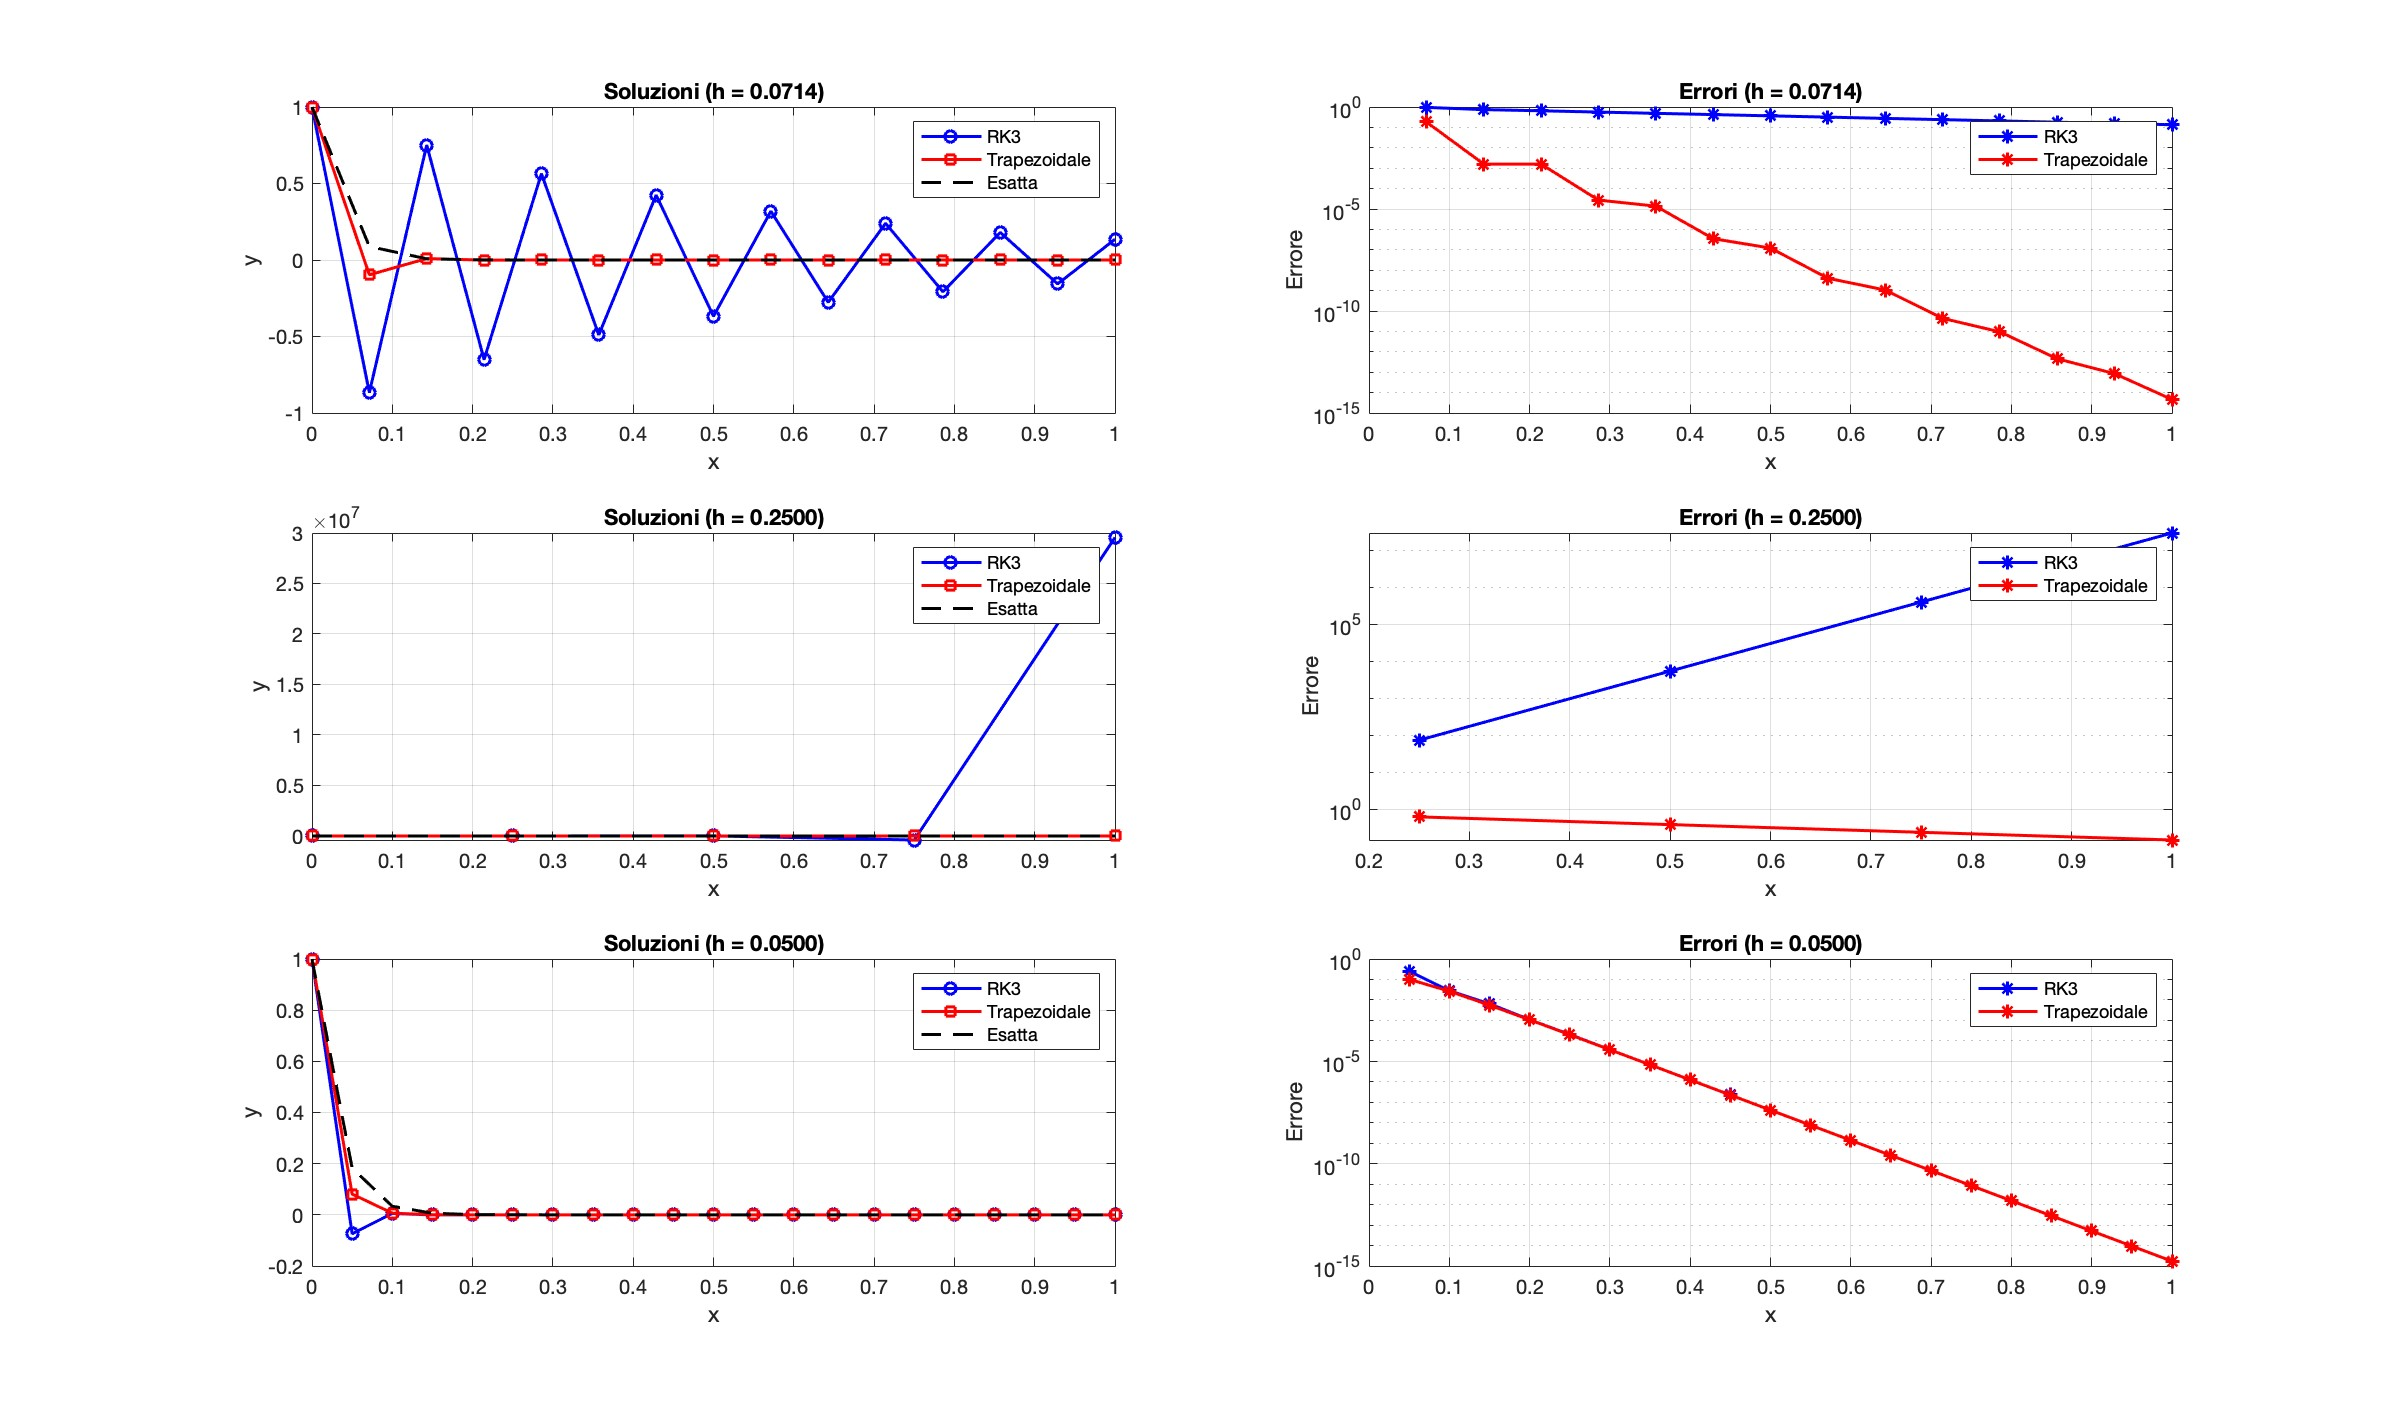
\includegraphics[width=1.2\textwidth]{images/fig5.jpg} 
  \caption{Le soluzioni e errori del metodo trapezzi e Runge-Kutta}
  \label{fig:funzione}
\end{figure}
\section{Esercizio 3}
\subsection{Consegna}
Preso dall'esercizio 8. Risolvere il seguente problema applicando il metodo shooting: 
\begin{align}
	y'' &= (2x/( x^2 +1 ))y'-(2x/( x^2 +1 ))+1\\
y(0)&=1.25 \\
y(4)&=-0.95 
\end{align}
(soluzione esatta $y = \frac{29x^3}{380} - \frac{x^2}{2} + \frac{87x}{380} + \frac{5}{4}$)
\subsection{Svolgimento}
Si pongono le variabili di stato:

\[
y_1(x) = y(x), \qquad y_2(x) = y'(x).
\]

Allora il sistema equivalente è:

\[
\begin{cases}
y_1'(x) = y_2(x) \\
y_2'(x) = \dfrac{2x}{1 + x^2} \, y_2(x) - \dfrac{2}{1 + x^2} + 1
\end{cases}
\]

con condizioni iniziali parametriche (shooting):

\[
y_1(0) = \frac{5}{4}, \qquad y_2(0) = s,
\]

dove \( s \in \mathbb{R} \) è la pendenza iniziale da determinare in modo che:

\[
y_1(4) = -\frac{19}{20}
\]
Per ogni \( s \), si integra il sistema nel dominio \( x \in [0, 4] \) (problema di Cauchy) e si definisce la funzione residuo:

\[
F(s) = y_1(4; s) - \left(-\frac{19}{20}\right).
\]

Si vuole trovare \( s \in \mathbb{R} \) tale che \( F(s) = 0 \).  
Per risolvere questa equazione scalare si possono utilizzare metodi numerici come:
\begin{itemize}
	\item il metodo di bisezione
	\item il metodo delle secanti
	\item il metodo di Newton
\end{itemize}
In questo caso, si utilizza il metodo delle secanti.  
Date due stime iniziali \( s_0 \) e \( s_1 \), si calcola iterativamente:

\[
s_{k+1} = s_k - F(s_k) \cdot \frac{s_k - s_{k-1}}{F(s_k) - F(s_{k-1})},
\]

fino alla convergenza, ovvero fino a che \( |F(s_k)| \) sia sufficientemente piccolo.\\
Per integrare il sistema, si utilizza il metodo di Runge–Kutta del quarto ordine (RK4).  
Dato un passo \( h \), e due punti consecutivi \( x_n \) e \( x_{n+1} = x_n + h \),  
si indica lo stato come un vettore colonna \( \mathbf{Y} = (y_1, y_2)^T \).  
Le formule del metodo RK4 sono:

\[
\begin{aligned}
K_1 &= f(x_i, Y_i), \\
K_2 &= f\left(x_i + \frac{h}{2}, Y_i + \frac{h}{2} K_1\right), \\
K_3 &= f\left(x_i + \frac{h}{2}, Y_i + \frac{h}{2} K_2\right), \\
K_4 &= f(x_i + h, Y_i + h K_3), \\
Y_{i+1} &= Y_i + \frac{h}{6} \left(K_1 + 2K_2 + 2K_3 + K_4\right).
\end{aligned}
\]
Il vettore funzione \(f(x, Y)\) rappresenta il lato destro del sistema differenziale, ovvero:

\[
f(x, (y_1, y_2)) = 
\begin{pmatrix}
y_2 \\
\displaystyle \frac{2x}{1 + x^2} \, y_2 - \frac{2}{1 + x^2} + 1
\end{pmatrix}.
\]
\subsection{Codice}
Nel codice è stato utilizzato \( i = 200 \) passi uniformi su \( [0, 4] \),  
quindi il passo di integrazione è:

\[
h = \frac{4}{200} = 0.02
\]
Tale valore è sufficientemente piccolo da rendere l'integrazione numerica molto accurata.
Si rende pubblico il codice (Es3, con le funzioni rk4, f\_ode, shooting\_residual):\\
Es3:
\begin{lstlisting}
close all
clear all
clc


% intervallo di integrazione
a = 0; 
b = 4;
i = 200;                        % numero di passi
x = linspace(a,b,i+1);           % griglia

% condizioni al contorno
y0 = 1.25;                       % y(0)
yb = -0.95;                      % y(4) (target)

% funzione residuo per la secante
F = @(s) shooting_residual(s, x, y0, yb);

% -------------------------------
% metodo della secante
s0 = 0;            % guess 1
s1 = 0.2;          % guess 2 (puoi cambiare)
tol = 1e-10;       % tolleranza
maxit = 50;

for k = 1:maxit
    f0 = F(s0);
    f1 = F(s1);
    s2 = s1 - f1*(s1-s0)/(f1-f0);
    if abs(s2-s1) < tol
        break;
    end
    s0 = s1;
    s1 = s2;
end
s_star = s2;
fprintf('Pendenza iniziale trovata: s = %.12f\n', s_star);

% -------------------------------
% integrazione finale con s_star
Y0 = [y0; s_star];
[Y] = rk4(@f_ode, Y0, x);

% soluzione esatta
y_exact = (29/380)*x.^3 - 0.5*x.^2 + (87/380)*x + 1.25;

% grafico
plot(x, Y(:,1), 'b-', 'LineWidth',1.5); hold on;
plot(x, y_exact, 'r--', 'LineWidth',1.5);
plot(4, yb, 'ko', 'MarkerFaceColor','k');
xlabel('x'); ylabel('y(x)');
title('Confronto soluzione numerica (shooting RK4) vs esatta');
legend('Numerica (shooting RK4)', 'Soluzione esatta', 'Location','Best');
grid on;
\end{lstlisting}
rk4:
\begin{lstlisting}
function y = rk4(f, y0, x)
% x sono il nodo iniziale + tutta la discretizzazione
% metodo di Runge-Kutta a 4 stadi di ordine 4
% y: matrice length(x) x n. di componenti di y

    y(1,:) = y0;       % inizializzo la prima riga
    n = length(x);
    for i = 1:n-1
        h = x(i+1)-x(i);

        K1 = feval(f, x(i),   y(i,:).');   K1 = K1(:).';  % --> riga
        K2 = feval(f, x(i)+h/2, y(i,:).' + h/2*K1.'); K2 = K2(:).';
        K3 = feval(f, x(i)+h/2, y(i,:).' + h/2*K2.'); K3 = K3(:).';
        K4 = feval(f, x(i+1),   y(i,:).' + h*K3.');   K4 = K4(:).';

        y(i+1,:) = y(i,:) + h/6*(K1 + 2*(K2+K3) + K4);
    end
end
\end{lstlisting}
f\_ode:
\begin{lstlisting}
function dydx = f_ode(x,y)
    % y(1) = y1 = y, y(2) = y2 = y'
    dydx = zeros(2,1);
    dydx(1) = y(2);
    dydx(2) = (2*x/(1+x^2))*y(2) - (2/(1+x^2)) + 1;
end
\end{lstlisting}
shooting\_residual
\begin{lstlisting}
% calcolo del residuo per la secante
function r = shooting_residual(s, x, y0, yb)
    Y0 = [y0; s];
    Y = rk4(@f_ode, Y0, x);
    r = Y(end,1) - yb;   % differenza con la condizione a x=b
end
\end{lstlisting}
\begin{lstlisting}[style=console]
	Pendenza iniziale trovata: s = 0.228947368687
\end{lstlisting}
Viene mostrata la soluzione insieme alla stima effettuata.
\begin{figure}[H]
  \centering
  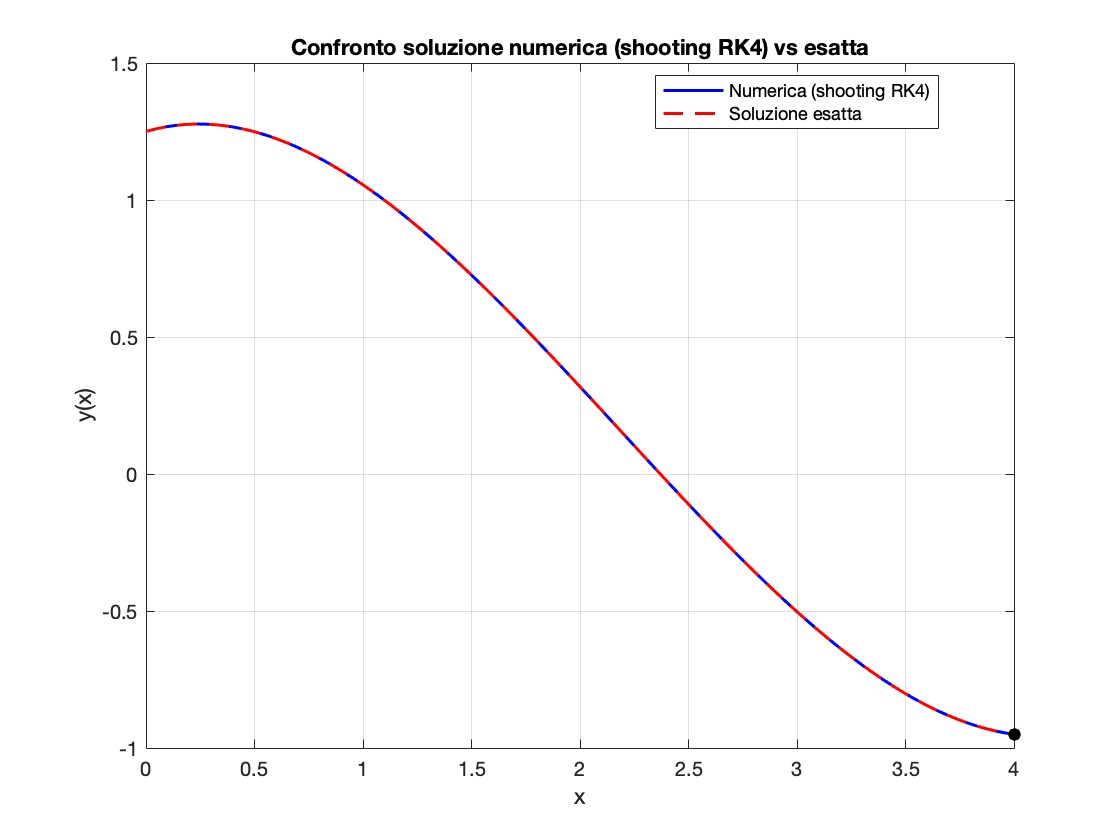
\includegraphics[width=0.7\textwidth]{images/fig6.jpg} 
  \caption{soluzione vs shooting rk4}
  \label{fig:funzione}
\end{figure}
Nel codice sono stati scelti come valori iniziali per il metodo delle secanti:
\[
s_0 = 0, \qquad s_1 = 0.2 
\]
(dove \( s_1 \) è una stima fornita nell'enunciato originale)\\
Riassumendo, il risultato finale è il seguente:\\
pendenza iniziale trovata (convergenza della secante):
\[
s^\star \approx 0.228947368421
\]
con questo valore di \( s^\star \), l'integrazione del sistema tramite RK4 fornisce:

\[
y_1(4; s^\star) = -0.950000000000,
\]
cioè il vincolo al bordo è rispettato con un errore numerico trascurabile (residuo \(\sim -3 \times 10^{-14}\)).
\section{Esercizio 4}
\subsection{Consegna}
Risolvere il modello predatore-preda
\begin{align}
	x'(t)=Ax(t)-Bx(t)y(t)\\
	y'(t)=Cx(t)y(t)-Dy(t)\\
	x(0)=3000 \qquad y(0)=120
\end{align}
con $A = 2$, $B = 0.02$, $C = 0.0002$, $D = 0.8$. Usare il metodo di Runge-Kutta nell’intervallo $[0, 5]$ e fare il grafico di $(x, y)$. Ripetere con $A = B = C = D = 1$ e $x(0) = 4$, $y(0) = 1$; risolvere nell’intervallo $[0,8]$; fare il grafico di $(x, y)$.
\subsection{Svolgimento}
Si crea uno script MATLAB che svolge il seguente problema e disegna dei grafici per $(x,y)$ per tutte e 2 le parti dell'esercizio. Es4 farà uso della funzione rk4 (per il metodo Runge-Kutta) e pred\_prey (per implementare il modello predatore-preda).\\
rk4:
\begin{lstlisting}
function y=rk4(f,y0,x)
% x sono il nodo iniziale + tutta la discretizzazione
% metodo di Runge-Kutta a 4 stadi di ordine 4
%%  struttura di y: matrice length(x)x n. di componenti di y
y(1,:)=y0;
n=length(x);
for i=1:n-1
    h=x(i+1)-x(i);
    K1=feval(f,x(i),y(i,:));
    x12=x(i)+h/2;
    K2=feval(f,x12,y(i,:)+h/2*K1);
    K3=feval(f,x12,y(i,:)+h/2*K2);
    K4=feval(f,x(i+1),y(i,:)+h*K3);
    y(i+1,:)=y(i,:)+h/6*(K1+2*(K2+K3)+K4);
end  
\end{lstlisting}
pred\_prey:
\begin{lstlisting}
% Definizione della funzione per il sistema predatore-preda
function dydt = pred_prey(t, y, A, B, C, D)
    x = y(1);
    y_val = y(2);
    dxdt = A*x - B*x*y_val;
    dydt = C*x*y_val - D*y_val;
    dydt = [dxdt; dydt];
end
\end{lstlisting}
Es4:
\begin{lstlisting}
%esercizio predatore-preda
clear all
close all
clc

% Prima configurazione: A=2, B=0.02, C=0.0002, D=0.8
A1 = 2; B1 = 0.02; C1 = 0.0002; D1 = 0.8;
x0_1 = 3000; y0_1 = 120;
h=0.01;
t_span1 = 0:h:5; % Intervallo [0,5] con passo 0.01

% Definizione della funzione con parametri specifici
f1 = @(t, y) pred_prey(t, y, A1, B1, C1, D1);

% Risoluzione con Runge-Kutta
sol1 = rk4(f1, [x0_1; y0_1], t_span1);

% Grafico della fase (x,y)
figure;
plot(sol1(:,1), sol1(:,2));
xlabel('Prede (x)');
ylabel('Predatori (y)');
title('Modello Predatore-Preda - Primo Caso (A=2, B=0.02, C=0.0002, D=0.8)');
grid on;

% Seconda configurazione: A=B=C=D=1
A2 = 1; B2 = 1; C2 = 1; D2 = 1;
x0_2 = 4; y0_2 = 1;
t_span2 = 0:h:8; % Intervallo [0,8] con passo 0.01

% Definizione della funzione con parametri specifici
f2 = @(t, y) pred_prey(t, y, A2, B2, C2, D2);

% Risoluzione con Runge-Kutta
sol2 = rk4(f2, [x0_2; y0_2], t_span2);

% Grafico della fase (x,y)
figure;
plot(sol2(:,1), sol2(:,2));
xlabel('Prede (x)');
ylabel('Predatori (y)');
title('Modello Predatore-Preda - Secondo Caso (A=B=C=D=1)');
grid on;
\end{lstlisting}
\subsection{Risultati}
Gli ultimi valori calcolati sono:
\begin{itemize}
	\item Caso 1 (t finale 5.0): $x(5)\approx3018.04$, $y(5)\approx120.35$
	\item Caso 2 (t finale 8.0): $x(8)\approx3.9764$, $y(8)\approx0.8235$
\end{itemize}
I seguenti grafici rappresentano i risultati ottenuti dalla soluzione numerica del sistema di equazioni differenziali del modello predatore-preda, utilizzando il metodo di Runge-Kutta del quarto ordine:
\begin{figure}[H]
  \centering
  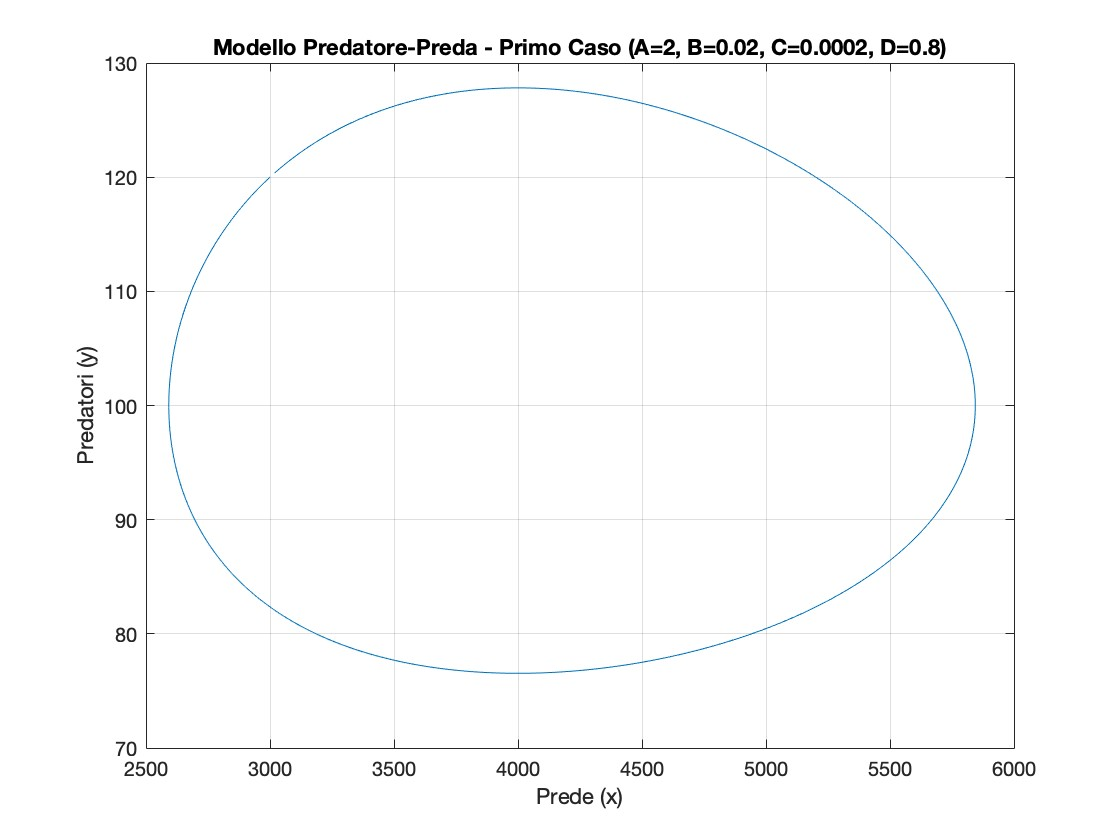
\includegraphics[width=0.7\textwidth]{images/Es4/fig1.jpg} 
  \caption{prima soluzione}
  \label{fig:funzione}
\end{figure}
Il grafico mostra un'orbita chiusa che rappresenta il ciclo delle popolazioni di prede e predatori
\begin{figure}[H]
  \centering
  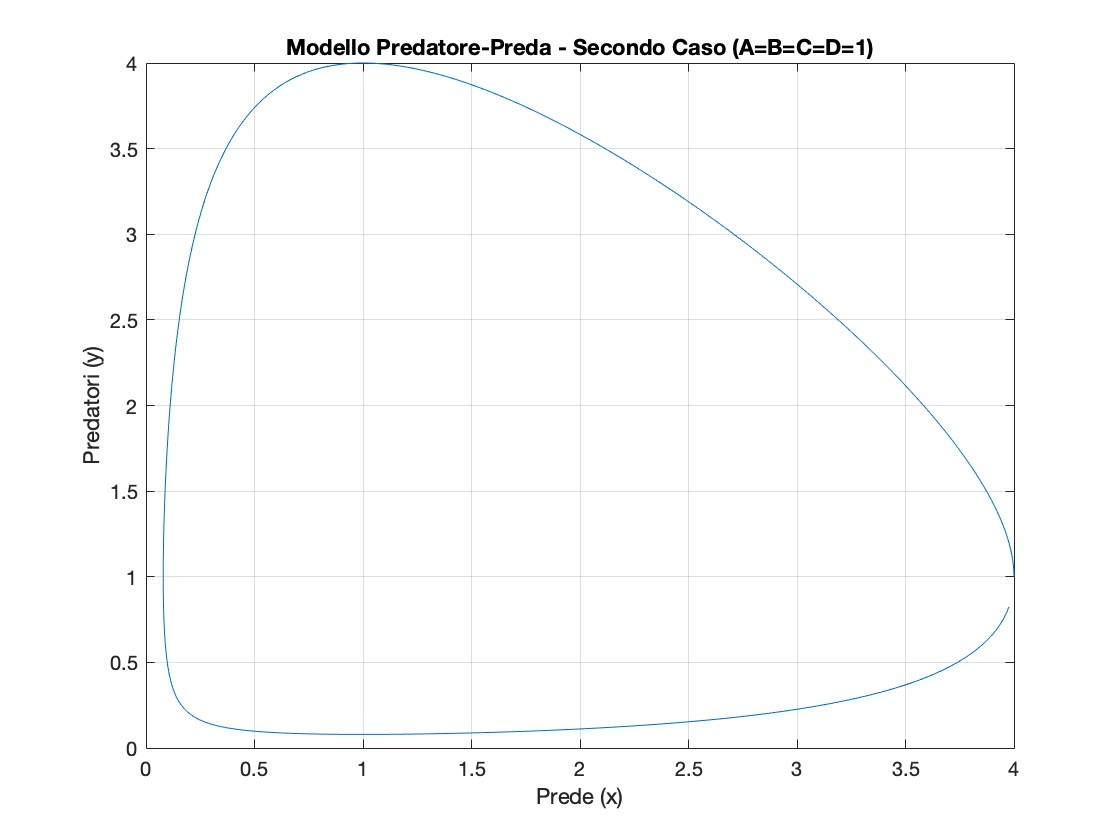
\includegraphics[width=0.7\textwidth]{images/Es4/fig2.jpg} 
  \caption{seconda soluzione}
  \label{fig:funzione}
\end{figure}
Anche in questo caso si osserva un'orbita chiusa, sebbene con caratteristiche diverse dovute ai differenti parametri
\end{document}